\documentclass[12pt]{article}
\usepackage[flushleft]{threeparttable}
%\documentclass[12pt]{elsarticle}
\usepackage{caption}
\usepackage{amsmath}
\usepackage[sort]{natbib}
\usepackage{geometry}
\usepackage{longtable}
\usepackage{setspace}
\usepackage{xspace}
\usepackage{graphicx}
\usepackage{lscape}
\usepackage{isorot}
\usepackage{booktabs}
\usepackage{float}
\usepackage[print,sectionbreak,panelright]{pdfscreen}
\usepackage{hyperref}
\usepackage{array}
\usepackage{amssymb}
\usepackage{siunitx}
\newcolumntype{H}{>{\setbox0=\hbox\bgroup}c<{\egroup}@{}}
\setlength{\textwidth}{6.5in}
\setlength{\textheight}{9.0in}
\setlength{\oddsidemargin}{0in}
\setlength{\topmargin}{0.0in}
\setlength{\headheight}{0in}
\setlength{\headsep}{0.0in}
\setlength\parindent{0pt}
\usepackage{subcaption}
\makeatother
\usepackage{babel}
\documentclass[english]{article}
\usepackage[LGR,T1]{fontenc}
\usepackage[latin9]{inputenc}
\usepackage{amsmath}
\DeclareMathAlphabet{\mathpzc}{OT1}{pzc}{m}{it}
\usepackage{hyperref}
\usepackage{listings}
\usepackage[utf8]{inputenc}
\hypersetup{
    allcolors=egyptianblue,
    citecolor=egyptianblue,
    colorlinks= true,
    linkcolor= egyptianblue,
    filecolor=egyptianblue,      
    urlcolor=egyptianblue,
}
\usepackage[colorlinks=true, allcolors=blue]{hyperref}%
\usepackage{nccmath}
\usepackage{mathtools}
\usepackage{appendix}  

% Custom colors
\usepackage{color}
\definecolor{deepblue}{rgb}{0,0,0.5}
\definecolor{deepred}{rgb}{0.6,0,0}
\definecolor{deepgreen}{rgb}{0,0.5,0}
\definecolor{orange}{rgb}{1,0.5,0}
\definecolor{egyptianblue}{rgb}{0.06, 0.2, 0.65}

\newcommand{\PVAS}[1]{\textcolor{red}{#1}}
\newcommand{\ian}[1]{\textcolor{deepred}{#1}}
\newcommand{\brendan}[1]{\textcolor{deepgreen}{#1}}
\newcommand{\trevor}[1]{\textcolor{deepblue}{#1}}
\newcommand{\russell}[1]{\textcolor{orange}{#1}}




% Default fixed font does not support bold face
\DeclareFixedFont{\ttb}{T1}{txtt}{bx}{n}{9} % for bold
\DeclareFixedFont{\ttm}{T1}{txtt}{m}{n}{9}  % for normal



% Python style for highlighting
\newcommand\pythonstyle{\lstset{
language=Python,
basicstyle=\ttm,
otherkeywords={self},             % Add keywords here
keywordstyle=\ttb\color{deepblue},
emph={MyClass,__init__},          % Custom highlighting
emphstyle=\ttb\color{deepred},    % Custom highlighting style
stringstyle=\color{deepgreen},
frame=tb,                         % Any extra options here
showstringspaces=false            % 
}}


% Python environment
\lstnewenvironment{python}[1][]
{
\pythonstyle
\lstset{#1}
}
{}

% Python for external files
\newcommand\pythonexternal[2][]{{
\pythonstyle
\lstinputlisting[#1]{#2}}}

% Python for inline
\newcommand\pythoninline[1]{{\pythonstyle\lstinline!#1!}}


\begin{document}



\title{GSE 580 Distribution of Price Changes: API Data

\author{Brendan Hoang 
\thanks{Cal Poly, Graduate Student, Department of Economics (email:
\tt{bhoang09@calpoly.edu})}
\and Ian Donovan
\thanks{Cal Poly, Graduate Student, Department of Economics (email:
\tt{idonovan@calpoly.edu})}
\and Trevor Luenser
\thanks{Cal Poly, Graduate Student, Department of Economics (email:
\tt{tluenser@calpoly.edu})}
\and Russell McIntosh
\thanks{Cal Poly, Graduate Student, Department of Economics (email:
\tt{rumcinto@calpoly.edu})}
}}


\maketitle


\begin{abstract}
%We use daily prices collected from online retailers in five countries
%to study the impact of measurement bias on three common price stickiness
%statistics. Relative to previous results, I find that online prices have longer
%durations, with fewer price changes close to 0, and hazard functions that
%initially increase over time. I show that time-averaging and imputed prices
%in scanner and CPI data can fully explain the differences with the literature.
%I then report summary statistics for the duration and size of price changes
%using scraped data collected from 181 retailers in 31 countries.

\trevor{Historically, it has been difficult to capture the degree and frequency that prices change.  Traditional methods, such as the use of scanner data, are presented on a weekly or quarterly basis and are often burdened by high costs in both time and wages.  In this paper we gather prices from a major online retailer for thousands of items daily to analyze price stickiness (the change in price, per item, over time) with a much higher degree of frequency.  We measure price stickiness by matching items over time and measuring the difference in price of the item from the period immediately prior.  Overall, our results indicate that online prices can be used to accurately measure prices over time, and that the distribution of price changes becomes more bi-modal over time, confirming the online price results in \citep{Cavallo2015}.
}

\end{abstract}


\noindent JEL: C9 \\
\noindent Keywords: GSE580, PPP, Purchasing Power Parity, Web-Scraping, Price Data.
\thispagestyle{empty}

\section{Introduction}
\label{introduction}
\setlength{\parindent}{5ex}
 %\ian{Researchers at the World Bank's International Comparison Program (ICP) are in need of recent price estimates for thousands of categories across hundreds of countries, this is clearly a daunting task. By using online data sources to supplement the large amount of manual data collection, researchers at the ICP would be able to greatly increase the speed and accuracy at which they are able to release Purchasing Power Parity reports. In this paper we examine the accuracy and reliability of using online data sources as a substitute for more labor intensive collection methods.}
 
 %Purchasing Power Parity estimates, despite their difficulty in derivation, provide practical real world benefit. PPP estimates are used to compare the economic well-being of countries across exchange rates. For example, if a researcher wants to know which countries incomes have grown the most over the last year they could use PPP estimates to compare income growth across countries. PPP lets the researcher make comparisons in terms of how many goods that country can purchase rather than how much is their currency worth. \citep{Moon2010}. 

%In past practices, price data had to be manually collected, creating a bottleneck for PPP calculation. As a result, price data may have already become outdated by the time it was used to draw PPP related conclusions. We will be avoiding this issue by utilizing Google's SerpAPI to access Walmart's price data in real time. 


\trevor{Price indices represent an important tool to both private and public sectors; from a business planning a product's pricing to NGOs measuring global purchasing power parities.  Measuring prices accurately is a significant concern since poor information can lead to poor investments.  While price collection has traditionally occurred in the field, or more recently through scanner data, new codes and the availability of online price data offer an enticing new direction for price index research.}

\trevor{Predominant issues in the collection of price data include the temporal and fiscal constraints of collection: collection in the field takes considerable time and person-hours, and scanner data may only be available as a weekly aggregate behind large pay-walls.  Online data is cheaper, easier, and far faster in its availability.  The ability to collect data on a daily basis offers another benefit: measuring price stickiness in terms of days rather than weeks.}

\trevor{Changes to current notions on price stickiness can have drastic policy implications.  The idea of prices being "sticky" is used to justify arguments that "changes in the money supply have an impact on the real economy, inducing changes in investment, employment, output and consumption" \citep{Wang2016}.  Stickiness impacts indices by misrepresenting price changes via current methodologies.  It is generally accepted that price stickiness is uni-modal, with prices largely remaining unchanged or showing little variation. Our own research, following that of \citep{Cavallo2015}, indicates that prices show a bi-modal distribution with slight increases and decreases that become more pronounced over time (\ref{fig:CavalloFig_1}).}


\subsection{Literature Review}



Past literature has discussed issues with the practice of using simple price data indices, such as the popularized Big Mac Index, to measure global price indices. Much of the goods contained in these indices cannot be traded internationally or contain incomparable service components, ultimately leading to issues in accurately comparing prices.  \citep{Taylor2004}. Despite these issues, price index estimates are used to analyze the effects of national culture such as individualism/collectivism, uncertainty avoidance, and economic capacity. Moreover, analysts can offer insight to retailers and mall managers on how to address variations in consumer behavior through price index estimation. \citep{Gilboa2020}. 


\ian{
One of the biggest issues surrounding the current large-scale price-index collection process is the enormous amount of data required to create accurate calculations. The International Comparison Program (ICP) collected price data for thousands of goods across 146 countries in 2005. The enormous amount of data that must be collected poses a complex problem with no single solution \citep{Angus2009}. In addition, the data collected fails to account for transportation costs and government taxes associated with each product in each country \citep{Pakko2003}.
}

\ian{
For example: collecting data for purchasing power parity (PPP) calculations is a cumbersome process that results in estimates being published years after the data has been acquired. The World Bank's International Comparison Program published PPP estimates for 2017 in 2020 \citep{Haishan2020}. A three year lag in the reporting of PPP estimates makes it difficult for decision makers to create relevant policies regarding a countries economic well-being. To give future decision makers up-to-date price data, researchers will need to make use of new technologies and methods to streamline the data collection process.
}

\trevor{
We discuss potential methods to improve the data collection process (e.g. Web scraping).  Web-scraping price data holds high desirability for a number of reasons, but the frequency of collection is a key aspect of potential benefits.  This may be most exemplified by the research of several National Statistics Offices on new methods of price data collection, such as the use of web-scraping supplemented by survey responses \citep{Bhardwaj2017} and the use of web-scraping supplemented by "copy-and-paste" techniques of online price data \citep{Polidoro2015}.   These methods have also been used to gather data in developing nations where data collection is more difficult or where countries opt-out of the World Bank International Comparison Program.
}

\trevor{
Web-scraped price data has proven viable for similar economic estimation techniques.  A significant issue with price data gathered online is its validity towards replicating established economic models.  Over the last decade several authors have shown that such data is indeed valid for use in predicting dis-aggregated consumer prices indices with a generally high rate of prediction \citep{Powell2018}.  Alberto Cavallo \citep{Cavallo2015} has also shown how scraped data can overcome time-averages and imputation method biases introduced through other data collection methods, specifically scanner and consumer price index data.  These contributions to the literature on web-scraped prices have established new methodologies for supplementing, and sometimes overcoming, traditional price data applications.
}

\trevor{
Without access to specific products presented in Cavallo's "Scraped Data and Sticky Prices" \citep{Cavallo2015} (due to the use of proprietary data) we seek to replicate those data with a subset of products, based on the categories presented in the Cavallo data set.  Our data come from daily scraped prices for 78 product-queries through Walmart's online retail store.  Queries represent the search term used in the website's search-bar.  These data are focused on products within the United States, in terms of US Dollars.  By using data across several industries and categories, we will study industry-level price variation; and due to the increased frequency of collection, we expect more price volatility than that seen from lower frequency (per month) data.
}

\trevor{
There are many benefits of Purchasing Power Parity estimates, but data collection and presentation is a time-consuming process with several barriers.  Advances in computing power and widespread data availability make the prospect of providing near real-time price index estimates very alluring.  While collection of expenditure data is beyond the scope of this paper, the collection of prices across several products over time can open a pipeline towards future developments in price index estimation.  Such data can allow for the formulation of consumer price indices estimates, which are conceptually similar to PPP estimates, with focus on the temporal and spatial changes in price, respectively \citep{Rao2001}.  By analyzing the "stickiness" of prices per product over time we can provide a platform from which to analyze concepts relevant to purchasing power parities such as the effects of externalities on individuals' purchasing power across time and space.
}

\trevor{
In Section~\ref{data} we will discuss the data presented by Alberto Cavallo in "Scraped Data and Sticky Prices" \citep{Cavallo2015}, as well as our own results via the collection of prices from Walmart. The~\ref{solution} section will describe the problems and proposed solutions that we encountered along the way. Section~\ref{analysis} will discuss the results of our findings with respect to the Walmart price data. Finally, the ~\ref{conclusion} section will tie our data and analysis together and explain gaps and limitations, as well as avenues for potential future analyses.\\
}

%\subsection{Literature Attribution}
%\begin{itemize}
%    \item Russell M. wrote paragraph one, part of paragraph two and edited/revised %the review.
%    \item Brendan H. wrote part of paragraph two and made revisions.
%    \item Ian D. wrote paragraphs 4-5 in red.
%    \item Trevor L. wrote paragraphs 3 through 7, colored deep blue with the "trevor{}" command
%     \PVAS{\item NEEDS ONE MORE CONNECTING PARAGRAPH HERE BEFORE CONCLUDING. 
%     \item TELL THE READER WHAT YOU'RE GOING TO DO TO TEST HOW REPLICABLE %CAVALLO'S AND OTHERS' METHODS ARE WITH WEBSCRAPED DATA PARTICULARLY OVER A SHORTER %TIME HORIZON.
%    \item STATE HOW YOU'RE GOING TO MEASURE "REPLICABILITY"? E.G. USING THE SAME %ITEM SEARCH TERMS AS CAVALLO FOR CERTAIN CATEGORIES, YOU'LL COMPARE XXX %METRICS/FIGURES USING HIS DATA TO YOUR DATA. \item THIS IS GOING TO SHOW WHAT? 
%    \item THE PREVIOUS TEXT IS GREAT. YOU CAN NOW TAKE IT OUT OF THE BULLET FORMAT %FOR THE NEXT ITERATION
%    }
%\end{itemize}  


\section{Data}
\label{data}

The data in "Scraped Data and Sticky Prices" \citep{Cavallo2015} are collected from the websites of 8 different large retailers from 5 different countries (Argentina, Chile, United States, Brazil, Colombia). Table~\ref{table:cavallo} describes the database of prices that \citet{Cavallo2015} uses for the US and the 4 other Latin-American countries studied. There are over 60 million daily price points that are used. Each of the 4 USA datasets represent prices from either a supermarket, convenience store, or electronics store. The datasets for the remaining countries all represent prices from a supermarket.  

Observations in the data set are collected on a daily basis, each observation represents the price of a particular good given by the category indicators on a particular day. The fewest number of observations of any country is the 4 million from Colombian supermarkets while the largest is 11 million for USA department stores. The fewest number of unique products from any countries also belong to Colombia and USA department stores is 4 thousand and the largest number was 94 thousand.

The \citet{Cavallo2015} data were collected via a program set to scrape prices at a set time daily.  A later version of this paper explains, generally, that several programs were used to scrape data at a set time, collating each observation as an individual product per day, parse the data into useful information, and store observations into a database in the format of one entry, per-product, per-day \citep{Cavallo2015}.  The products are given unique product IDs to reference and group over time, as well as product categories that can be used to analyze changes at the product-category level.  Our data are collected similarly, using Google's SerpAPI application, which aggregates prices from Google Shopping search results in 21 countries for 5 search-query parameters, and collects the first 20 entries, to 2,100 observations per day.  We also used the SerpAPI application to pull data from Walmart to collect price, title, product identifiers, and various metadata.  An abbreviated version of the code (offering a limited query parameter) uses 18 search-query strings, totalling approximately 675 observations per day.  An expanded version of the Walmart API uses 78 search-query strings to search for products, pulling approximately 3,000 observations per day.  Under ideal conditions we will run the API code for a considerable period of time to analyze long-term trends in the price data, how it compares across countries, and compare the results to both Cavallo's CPI stickiness results (which analyzed price-percentage-changes over time) and PPP estimates.


\begin{table}[] \caption{API Data}
\centering
\begin{tabular}{lcc}
\multicolumn{3}{l}

                                                            \\ \hline
                     & \multicolumn{1}{l}{Google Shopping} & \multicolumn{1}{l}{WalmartAPI (Abbreviated)} \\ \hline
Queries^{a}              & 5                                                    & 18                                              \\
Locations^{b}            & 21                                                   & 1                                               \\
Observations (daily) & 2100                                                 & 677                                             \\ \hline
\end{tabular}\\
\scriptsize \trevor{^{a} \text{queries are strings acting as search-terms in the search-bar}}\\
\scriptsize \trevor{^{b} \text{locations are strings used to reference a geographical server from which the search takes place}}
\end{table}
\label{table:scrape}

There are eight unique data sets: USA1, USA2, USA3, USA4, Argentina, Brazil, Chile, and Colombia. USA1 contains 9 million daily price records for 24 thousand items from supermarkets in the US. USA2 contains 10 million price records for 94 thousand items from department stores in the US. USA3 contains 4 million price records for 22 thousand items in drugstores and convenience stores in the US. USA4 contains 5 million price records for 30 thousand items in electronics stores. The remaining data sets record price data for items in supermarkets exclusively. Argentina contains 11 million price records for 28 thousand items. Brazil contains 10 million price records for 22 thousand items. Chile contains 10 million price records for 24 thousand items. Colombia contains 4 million price records for 9 thousand items.


\begin{table}
\centering
\scalebox{1}{
  \begin{threeparttable}
    \caption{Database Description (Table 2 of \citet{Cavallo2015})}
     \begin{tabular}{llllll}
        \toprule
         & \( US \) & \( Argentina \) & \( Brazil \) & \( Chile \) & \( Columbia \) \\
        \midrule
Retailers                       & 4                                 & 1                             & 1                          & 1                         & 1                            \\
Observations (millions)         & 28                                & 11                            & 10                         & 10                        & 4                            \\
Products (thousands)            & 172                               & 28                            & 22                         & 24                        & 9                            \\
Days                            & 865                               & 1,041                         & 1,026                      & 1,024                     & 992                          \\
Initial Date                    & 03/08                             & 10/07                         & 10/07                      & 10/07                     & 11/07                        \\
Final Date                      & 08/10                             & 08/10                         & 08/10                      & 08/10                     & 08/10                        \\
Categories                      & 49                                & 74                            & 72                         & 72                        & 59                           \\
URLs                            & 16,188                            & 993                           & 322                        & 292                       & 123                          \\
Total missing observations (\%) & 37                              & 32                            & 26                         & 33                        & 22                           \\ \hline
        \bottomrule
     \end{tabular}
     
    \begin{tablenotes}
      \small
      \item Retailers: The number of retailers in each country from which price data was scraped
      \item Observations: Total number of price observations
      \item Products: Total number of unique items in the data
      \item Days: Total number of days that data was scraped in each country
      \item Initial Date: Initial date of price-data scraping
      \item Final Date: Final date of price-data scraping
      \item Categories: Total number of COICOP categories into which products fall
      \item URLS: 
      \item Total Missing Observations: Percent of observations that are missing price data
    \end{tablenotes}
  \end{threeparttable}
  }
\end{table}
\label{table:cavallo}



There are implicit biases associated with web-scraped data. \citet{Cavallo2015} specifically references three primary disadvantages of scraped data: a much smaller representation of product categories, sources being limited to large multi-channel retailers, and lack of information on quantities sold \citep{Cavallo2015}.  He also describes the second point as potentially falling victim to sampling bias.  For our own data, sampling bias represents a significant concern due to search-engine-optimization, paid advertising, and the weight given to product views and ratings.  

Reporting bias and exclusion bias go hand-in-hand with the inability to collect data from local markets, small retailers, and other potential sellers whose data is not readily available compared to major online retailers. Only a limited number of countries have been represented in either \citet{Cavallo2015} or our own data.  In our own case, we are limited to countries that are available in Google's search API, and countries in which Walmart operates.  More generally, it will often be difficult to acquire data from nations such as Iran, North Korea, or Myanmar who restrict or sever access to digital marketplaces.

As previously mentioned, excluding a large number of countries in our data sample may lead to biased price comparisons (caused by sampling bias) when extrapolating the web-scraping data collection methods to more countries and products. These potential biases may wane as purchasing habits across the world trend towards larger retailers and developing countries further digitalize. 

There are likely to be some unavoidable consequences from using the \citet{Cavallo2015} data as the prices from the Latin American countries are all derived from supermarkets, and therefore only represent a basket of goods that can be bought at such a retailer. This resulting exclusion of a significant subset of goods and services provided by smaller (and potentially more regionally popular) retailers may lead to difficulty in arriving at accurate price comparisons.  Additionally, the \citet{Cavallo2015} paper  mentions that the majority of transactions are still handled offline in many countries, making online prices not a fully accurate depiction of what people are actually paying for goods in the respective countries. Moreover, residents of other countries likely have varying purchasing habits in terms of where they buy goods, raising potential room for concern caused by our focus of big name retailers. Our original data suffers the same potential for harm as it is limited to a necessarily small sample of goods and countries. 


\vskip 10 pt


%\PVAS{PROFESSOR VASILAKY'S COMMENTS WEEK 5 (29/30):
%GOOD RE-WRITES. FIX THE TERMONOLOGY ON SCRAPING VERSUS APIS.}







% \PVAS{PROFESSOR VASILAKY'S COMMENTS WEEK 4 (40/40):
% DATA SECTION LOOKS GOOD. YOU CAN TAKE IT OUT OF BULLETED FORMAT. YOU'LL JUST NEED TO UPDATE THE TABLES AS YOU GET CLOSER TO WHAT YOUR ACTUAL DATA WILL LOOK LIKE. IT WOULD ALSO BE GOOD TO HAVE YOUR TABLE OF SCRAPED DATA BREAK QUERIES DOWN BY CATEGORY AND SEARCH TERM AND INCLUDE A COLUMN FOR DURATION }



%Data Attribution\\
%\begin{itemize}
%\item Ian D wrote the sections on Who/What does your data represent, and How many observations. Also formatted and edited each paragraph.

%\item Brendan H added details to the Biases sections and wrote revisions.

%\item Russell M wrote wrote the sections on where does the data come from, the potential harm of the data, and the implications of the biases.

%\item Trevor L wrote the sections on Data Representation, Data Collection, and Biases, and drafted Tables 1 and 2.
%\end{itemize}

%Data Section Instructor Comments (inline):\\
%\begin{itemize}
%    \item [\PVAS{DEFINE STICKINESS RESULTS. I DONT' THINK YOU CAN CALCULATE PPP}]  
%    \item \PVAS{WHERE EACH ENTRY IS PER PRODUCT PER DAY}  
%    \item \PVAS{OUR DATA ARE}  
%    \item \PVAS{WHICH}  
%    \item \PVAS{AND COLLECTS}  
%    \item \PVAS{TO}   
%    \item \PVAS{I THINK I'VE SAID THIS A FEW TIME ALREADY, BUT YOU ARE NOT SCRAPING DATA WHEN YOU USE AN API. PLEASE CHANGE THIS!}   
%    \item \PVAS{PULL}   
%    \item \PVAS{AGAIN, YOU ARE NOT RUNNING SCRAPING CODE}   
%    \item \PVAS{DEFINE A QUERY, AND A LOCATION. IS ONE QUERY A SEARCH FOR ONE PRODUCT GIVEN A LOCATION? }  
%    \item \PVAS{LABEL YOUR TABLES AND REFERENCE THEM. }  
%    \item \PVAS{DEFINE ALL YOUR VARIABLES HERE PEDANTICALLY.}  
%\end{itemize}


\section{Problem description}
\label{solution}


\brendan{ 
In past literature on price stickiness, authors have discussed how sampling and measurement error affect price statistics. In our paper, we hope to highlight common associated with measurement error in the context of calculating the price changes.}
\trevor{These measurement errors can negatively impact accuracy in common and influential price indices, including Consumer and Producer Price Indices (CPI) and Purchasing Power Parity (PPP).}   \russell{Price data collection for price index estimates has proven to be a strenuous task due to difficulties in extracting the high volume of data required to draw meaningful conclusions.}

\subsection{Cavallo Replication} 

\russell{Cavallo has explored issues such as measurement error in price data collection, and will partially replicate Cavallo's analysis from \citep{Cavallo2015} in which he compares online price data to scanner data to evaluate biases on measuring price stickiness. Notably, Cavallo shows that although daily online data captures more price fluctuations, it is found to be stickier than scanner data when evaluated at the same time interval. He attributes this to the sampling bias present in scanner data caused by supplemental time averages and imputations that in turn falsely reduces the duration of price changes. Building upon this, we will be evaluating price changes utilizing an API as opposed to web-scraped online price data or scanner data. 
Through a density plot visualization, based upon Figure 1 in Cavallo's paper, we will be able to observe the variation of price changes between our shorter-termed data set of Walmart's online prices and Cavallo's longer-termed data set of online US prices . Additionally, we will subset Cavallo's online price data to a 14 day period and create a similar plot to compare his results if his time horizon was the same as ours. We will also include a similar summary table to Cavallo's Table 2 in order to provide contrast between the two data gathering methods (API and Web-Scrape), as well as display the depth of our collection.  
In addition to providing insight towards the effectiveness and feasibility of API derived price data of a single large retailer, our method will also show its applicability in contributing to short term analysis of price changes.
}
\subsection{Difficulties}

\russell{ It is difficult to derive a feasible data collection method that is both accurate and efficiently.}  \brendan{Historically speaking, analysts have encountered some difficulties when certain scanner prices could not be expressed in whole cents. The issue of "fractional prices" will be addressed in the paper by the usage of intermediary data collection methods.}  

\trevor{There are differences in purchasing preferences and behaviors across, and even within regions.  As we have seen in our own data collection, prices are often difficult to acquire, or may be so variable as to make accurate product pricing difficult to ascertain without related sales data.  Differences in item quality can potentially be significant across markets.  Unique product identifiers, such as SKU and UPC codes, can change over time leading to a comparison of different products, or continuing collection for the same product data, to become inaccurate.}  \russell{ By the time the data has been used to create estimates for 
%\PVAS{INDICES LIKE PPP OR CPI}
indices such as Purchasing Power Parity or consumer price indices, it may already have become outdated. 
}

\subsection{Overview of Solutions}

\trevor{By using prices pulled from Walmart's API, we overcome the need to use intermediary sources of data collection, such as scanner data and in-person records.  Walmart's online prices are standard across regions within the United States, overcoming concerns about regional pricing differences.  Large collections of daily data allow us to collect prices from a large number of items per query, allowing us to disregard observations without price information.  In trials, a negligible number of observations have been lost (performing the initial test on data collected May 8, 2021, 1 of 2852 observations did not have price data, or 0.035063113\% of observations).  Items sold by Walmart online are also standardized across regions, negating the potential for quality differentiation across regions.}  

\trevor{Having access to two forms of unique product identifiers and product titles allows us to potentially compare three identifying labels to ensure products are the same over time, forgoing issues such as changing SKU or UPC codes.}

\trevor{We seek to increase the availability and quantity of price data by running data collection code on a daily basis.
}  
\russell{We begin our approach to these issues by utilizing python to access Google's SerpAPI. Our basket of goods contains 11 categories of items that are common across countries \footnote{Foods,Drinks,Home Improvement,Home and Furniture,Toys and Games,Dry Goods,Electronics,Clothing and Accessories,School and Office,Health,Entertainment}}  

\russell{The prices are gathered from Google's SerpAPI platform, and are accessed through Walmart's online store using the Walmart engine. Our collection of real time daily prices will allow us to create a data set that can be used to analyze price changes across time at a higher frequency than that of CPI or scanner price data. Automating the data collection in this fashion negates the issue of letting the data become outdated during analysis. Being able to work with current price data will create a significant advantage in overcoming the prior mentioned difficulties in price data collection.}




\subsection{Data Collection Method}
\trevor{
The code in Appendix~\ref{appendixA} - Appendix~\ref{appendixF} shows how the data were collected from Google's SerpAPI platform using the Walmart engine.  An abbreviated version was used to start collecting data on April 28, 2021, while an expanded version (including several new queries) was started on May 5, 2021.  Minimal changes were used to gather data from Google Shopping through the SerpAPI Google Search engine.
}

\ian{After collecting and cleaning the price data we calculate average price changes for each day in the data. We begin by calculating the average price for each day, next we take the average price of the following day and subtract off the current price before dividing this quantity by the current price. Using this formula we are able to derive daily average price changes for online products in the US. Finding a distribution of price changes that is similar to the distribution found by Cavallo, would provide evidence to support the hypothesis that online prices can be used to supplement physical price data.}
  
  
  
%\subsection{Problem and Solution Attribution:}
%\begin{itemize}
%\item \ian{Ian} wrote the R code to extract price data.
%\item \brendan{Brendan} wrote the main script from the original Cavallo script and contributed to sections in the first paragraph of the Problem Description section of the paper, and made revisions.
%\item \trevor{Trevor} wrote the data collection codes, wrote the read me .txt file, wrote the variable information .txt file, wrote the collection and concatenation .txt file, added sections to the problems section, and added sections to the solutions section.
%\item \russell{Russell} wrote the table 2 replication code, sections in the problem section, sections in our own solutions, and  sections in the replicated cavallo solutions 
%\end{itemize}

%Instructor Comments:
%\begin{itemize}
%    \item \PVASP{MEASUREMENT ERRORS IN PRICE STATISTICS CAN INFLUENCE THE ACCURACY OF PRICE INDICES SUCH AS PURCHASING POWER PARTIY, CONSUMER PRICE INDICES, XXXXX.} 
%    \item \PVAS{PROFESSOR VASILAKY'S COMMENTS WEEK 6 56/60\\
%    Overall, good work. See the comments I left in the margin. Move the explanation regarding Cavallo's work up. It can be introduced sooner. It also  needs a bit more explanation. Describe the paper you are referencing. What does it aim to do and why?  What parts of that paper - tables/figures - are you replicating? Fix the references about scraping where noted. Move the code into an appendix section and reference it, rather than inline.\\
%    For the file structure - some part needs finishing. The descriptions of the files should be listed INSIDE the file structure, rather than a few that are described above. What is Walmart abbreviated versus expanded? Where should the user be changing their API key? } 
%\end{itemize}

\section{Results}
\label{analysis}
\ian{We begin by comparing the price distribution found by Cavallo in Figure~\ref{fig:Cavallo_dist} to the price distribution we obtained with our aggregated data in Figure~\ref{fig:price_dist}. Immediately, we see that there is a higher concentration of price changes around 0 in our distribution when compared with Cavallo's.}
\trevor{However, comparing a subset of Cavallo's data, from April 28, 2010 to May 23, 2010 to coincide with our own data, we see a similar distribution of price changes across categories.  Immediately noticeable is how the increased number of categories and products flattens the density compared to our own results.}
\ian{The maximum price decrease in our sample was -10\% while the maximum price increase was about 3\%. When comparing the variability of the two distributions we see less variance in our sample and a left skew. When compared with Cavallo's results, our aggregated price data more closely matches the CPI imputation data rather than the online price data. To make a more accurate comparison to Cavallo's data, we also plot the average price changes for a 14 day sub sample from May 1st, 2008 until May 14th, 2008. The distribution of price changes for the sub sample can be seen in Figure~\ref{fig:sub_dist}. Comparing the sub sample distribution with the distribution from the API data we can see that the sub sample has less variance and has more observations around 0. While the size of the price changes are not very similar the shape of the distributions are fairly comparable considering this is only looking at a 14 day window.}

\trevor{It is likely that scanner data provides misleading results from smoothing of the data.  Prior literature had shown price changes to largely be uni-modal around zero, but Cavallo argues that the true distribution is bi-modal, with a positive and negative mode.  Figure~\ref{fig:CavalloFig_1} shows a subset of Cavallo's scraped prices compared to both a simulation of the data averaged by week and scanner data obtained by AC Nielson for the same retailer.  Cavallo notes that the weekly averaging of prices in the simulated and scanner data reduces the affects (and visualization) of large price changes.  Coupons and loyalty cards may act to further smooth the price changes by providing consumers with lower prices than those posted, affecting the scanner data but not scraped prices.  
We should also note that prices collected from our own API do not account for the possibility of temporary changes in prices due to a range of factors, such as overstocking, expirations, promotions, or new product launches.  Several observations in our data indicate massive changes, such as discounts in medicines, toys, and books that may be explained by expiration, new models, or lack of demand, respectively, or, drastic increases in prices that are not so easily explained.}
\trevor{It is difficult to capture the external validity of these findings.  Returning to purchasing power parities, it would be necessary to capture these data across borders; the Walmart price data focuses on US prices at a macroscopic level.  Time is also a factor that we hope to expand in the future; current events, such as mask mandates and social distancing orders, likely play a large role in daily price changes specific to region.  Walmart, one of the largest retailers in the world, let alone the US, may not capture how prices change for smaller retailers, especially those limited to intra-national or intra-regional markets.}

\subsection{Depth of Raw API Data}

\begin{center}
\begin{table}[hbt!]
\caption{Walmart API Data Summary}
\label{tab:my-table}
\begin{tabular}{@{}|ll|@{}}
\toprule
\tabcolsep = 0.07cm
\textbf{Walmart Data (US)}               & \textbf{Value} \\ \midrule
\textit{Start Date}                      & 4/27/21        \\
\textit{End Date}                        & 5/22/21        \\
\textit{Days}                            & 23             \\
\textit{Total Missing Observations (\%)} & 6.8            \\
\textit{Unique Products}                 & 5412           \\
\textit{URLS}                            & 8501           \\
\textit{Observations}                    & 53905          \\
\textit{Unique Categories}               & 11             \\ \bottomrule
\end{tabular}
\end{table}
\end{center}

\russell{ Table 3 presents the raw results of our data collection method across all product categories. There are 6.8\% of the 53,905 total price observations missing due to either items being out of stock or flaws with the Walmart API. Examining this further, we found that these price absences do not last for more than a few days. Compared to Cavallo's web scraping method, our usage of an API has produced less missing observations (by percentage of total observations). With more time to collect data however, the overall missing observation percentage may more closely align with Cavallo's results. In table 4 we further examine our sample divided into 5 sectors based on those commonly used for the creation of price indices. Most notably, the Food and Drinks sector has 20.53\% of its total observations missing, possibly due to supply shocks at the time of our data collection.}



\begin{center}
\begin{table}[hbt!]
\small
\tabcolsep = 0.07cm
\caption{Summary by Sector (Walmart API US)}
\label{tab:my-table}
\begin{tabular}{|l|lllll|}
\hline
\textbf{} & \textit{\textbf{Food/Beverages}} & \textit{\textbf{Electronics}} & \textit{\textbf{Household Goods}} & \textit{\textbf{Clothing}} & \textit{\textbf{Health}} \\ \hline
\textit{\textbf{Average Price (Dollars)}} & 15.06 & 293.47 & 58.79 & 16.15 & 13.31 \\ \cline{1-1}
\textit{\textbf{Unique Products}} & 1307 & 422 & 1236 & 1007 & 309 \\ \cline{1-1}
\textit{\textbf{URLS}} & 2054 & 573 & 2008 & 1253 & 842 \\ \cline{1-1}
\textit{\textbf{Total Missing (\%)}} & 20.53 & 0.0 & 1.33 & .21 & .07 \\ \cline{1-1}
\textit{\textbf{Observations}} & 13381 & 4335 & 14110 & 5137 & 4248 \\ \hline
\end{tabular}
\end{table}
\end{center}

Even with a few weeks and roughly 55,000 observations sampled, we were still able to witness noticeable price changes that could be represented graphically in Figure 2. Our ability to derive results of this fashion should be viewed as a positive in terms of evaluating the feasibility of our API data collection method.



%\subsection{Week 7 Attributions}
%\begin{itemize}
%\item \ian{Ian} Started the results section, organized the price data, and created Figure 2. 
%\item \brendan{Brendan} Worked through the Cavallo code to replicate Figure 1. 
%\item \trevor{Trevor} Worked on instructor's comments in the Problem section, wrote part of the Results section, continued collecting data, and worked on troubleshooting code and documentation.
%\item \russell{russell} Worked on comments in the problem section, created updated summary table in the results section (table 3), and wrote about table 3 in the results section.
%\end{itemize}

%\PVAS{Professor Vasilaky's Week 7 comments 35/40:\\
%Overall - good start to the results section. Certain points need more clarity on what Cavallo did, and what he found, and how your results differ. I left comments in the margins and summarize them below, as well as a suggestion for another graph comparing your data to Cavallo's. 
%\begin{itemize}
%\item Problem Description 
%\begin{itemize}
%\item Make sure you define price stickiness. Is it just the percent change in prices for a product day to day?
%\item The problem description needs more explanation of what Cavallo is attempting to do by plotting price changes between online data and scanner data. I left note as to where you can do that. 
%\item The intention of the Cavallo paper is to compare scanner data to online data - not to do away with scanner data. In particular, he wants to show that the ways in which scanner data had previously been "filled out" in past papers gave an erroneous picture of price stickiness. Online data, he found, was stickier - and your group should explain why - which led to that bimodal distribution of price changes of online data. 
%\end{itemize}
%\item Results
%\begin{itemize}
%\item Clearly state why the distributions of the two price sources differ, and explain which one Cavallo believes is the "true" distribution. 
%\item To make a more fair comparison of the Cavallo data with your data, take a 14 day snippit of his data and plot it and compare it to your 14 day period of data. 
%\item If the distribution of price changes for your online data differs from Cavallo's then you should give some explanation as to why you think that is. 
%\end{itemize}
%\end{itemize}
%}
\section{Discussion and Conclusion}
\label{conclusion}

%\noindent{Paragraph 1 (Problem/Approach)} \\


\brendan{Accurate price data is crucial for comparing economic capacities between countries with different exchange rates via price indices, but this data is not easily obtainable and often requires methods to supplement missing data. The process of gathering price data typically involves a significant amount of manual data collection through inflation indices and scanner data. Data sets collected via these means can lead to measurement errors and biases due to imputation methods used to fill in price gaps. This issue, as presented by \citep{Cavallo2015}, is addressed by using online data sources to increase the accuracy in measuring price stickiness and creating price indices. Moreover, online price data allows researchers to create insight on current price data, as opposed to price data that has potentially already become obsolete. Using these methods, researchers can create customized data sets to more effectively analyze price stickiness across products, sectors, and countries. \citep{Cavallo2015} emphasized that previous empirical studies using common indices often include imputed prices as substitutes for temporarily missing products. By collecting online data through SerpAPI and analyzing the resulting distributions, we find that using online data to measure price stickiness yields a bimodal distribution that differs from the scanner data distribution. We argue this is due to our API collected data being free of imputation methods or averaging that would otherwise cause price change estimates from the tails to be moved towards the center of the distribution curve.  In the short run however, we see a more unimodal distribution. This may be the case that prices are more resistant to change in the short run, as firms can incur expenses when changing prices(menu costs).} 


%\noindent{Paragraph 2 (Summarize Results)} 
\brendan{The results from \citep{Cavallo2015} indicated that previous literature on price stickiness used scanner and CPI data to fill out missing data points. In this paper, we used online daily price data from a large retailer accessed from Google's serpAPI platform to run search-query terms and collect weekly product prices from Walmart. We study the magnitude of price changes to compare the resulting price data distribution to that from \citep{Cavallo2015}. We implemented R and Python scripts to parse and sort the scraped observations and create graphical representations. Overall, our findings suggest that data collection methodologies stemming from online data as opposed to scanners can increase the accuracy of price stickiness analyses - online data is stickier than scanner data, and prices are stickier in the short run than long run. Compared to the data sourced from scanners, the online data yields a distribution that more closely resembles a bimodal distribution of price changes. Examining the beginning of our data collection, we find there to be a more unimodal distribution that is potentially due firms resisting price changes.  As a result, our method suggests that data from online sources such as APIs can reasonably be used in international price indices to compare baskets of goods and purchasing power parities.} 


%\noindent{Paragraph 3 (Caveats/Limitations)} 
\brendan{Compared to \citep{Cavallo2015}, our model did not have access to scanner data.} 
\trevor{In addition, our data lacks the scope of time, daily observations, and total categories, all of which can be remedied with continuing work.  Broader limitations are the lack of information regarding product expenditures necessary to calculate price indices, as well as price data from other countries.  Although the data provide significant steps towards the calculation of indices that do not rely on expenditure data, we still seek data from foreign marketplaces such as Mercado Libre and Jumia.  Access to such market data would prove invaluable to future work on price measurement.} 


%\noindent{Paragraph 4 (Future Work/Applications)} 
\brendan{Our research poses several possibilities for future empirical studies regarding price stickiness in the monetary transmission mechanism. We found that using API data could feasibly improve the efficiency of estimating purchasing power parities. Through our research, we deduced that previous reports and literature underestimated price stickiness due to sampling measurement errors. However, our paper presents numerous avenues for future study, such as the effectiveness of daily online price data in informing policy makers on capital allocation decisions. With the ability to create accurate daily price indices, global markets would be able to be intently monitored constantly. }



%\PVAS{\\Professor Vasilaky's Week 8 comments\\
%THROUGHOUT THE PAPER:\\
%- Replace API or SerpAPI with price data from a large online retailer (except in the data section. Do explain the Application Program Interface (API) in the data section). As a reader, I care about where the data are coming from. API doesn't tell me that, and many people don't know what API stands for or what it is. \\
%- Everywhere where you say Cavallo's paper should be replaced with \citet{Cavallo2015}\\
%- In general, try to replace PPP with more general terms like price indices throughout the paper. Previously, it seemed like we would get back to PPP, but that's not really the case, so when possible, do away with the specifics about PPP, I'm not asking you to add anything. Just try to lighten the discussion of PPP as an outcome of the paper, since it's not really an outcome of the paper anymore. But you can certainly relate the measurement of price changes back to price indices more generally (PPP, CPI, etc,). \\
%ABSTRACT (150 words only). \\
%The abstract goes far too deep into details.  The first sentence should state the problem you're studying regarding price stickiness or price measurement - namely capturing the degree and frequency with which prices for goods change. Tell us why this difficult to capture and why it matters?\\
%- No need to mention the World Bank or the assignment they gave you. You're situating the larger problem at hand here. Think of this as an academic paper rather than a consultancy deliverable.\\ 
%- In the second sentence should tell us how you will measure price stickiness.\\ 
%- Your results should discuss how the distribution of price changes changes with the duration of your price data collection. That is interesting. How does that compare to Cavallo's online data results versus his scanner data results?\\
%INTRODUCTION.\\
%The introduction is thin as it stands.\\
%First paragraph.The introductory sentence should state the global problem (not what the WB unit wants).\\ Why does measuring prices accurately matter? Why does price stickiness matter for estimating indices? What bearing do price indices have on decision making? Speak to the big overarching economic questions.\\
% Edit this paragraph and the lit review and replace PPP with more general terms like "price indices," since your paper does not deal with PPP anymore. 
%Second paragraph. In the second paragraph you should discuss what the specific issues are in collecting and measuring prices. You should look to the Cavallo paper for the past literature that has worked on this.\\
%CONCLUSION. \\
%Overall - try to avoid using terms and words that are not defined or don't add to your explanation of what you actually did. There are several instances of this,  and I've tried to point them out (e.g. computational imprecisions, microfoundations, etc. ) Avoid sentences (in particular, paragraph 4 could be removed or edited) that don't tell the reader anything new. \\
%Again, you can generalize the discussion to price data and their importance in price indices (rather than PPP) since this paper does not go into PPP calculation.\\
%Remove ICP World Bank. \\
%Your conclusion should summarize the following:\\
%-why price stickiness or measuring price\\ changes is important \\
%-why it's difficult to measure\\
%-what Cavallo did \\
%-what you add to Cavallo's paper, which is to study how the distribution of price changes (stickiness) changes over time, and your explanation for why that distribution changes. That's interesting!\\
%ABSTRACT 16/20\\
%INTRODUCTION 15/20\\
%CONCLUSION 18/20
%}






\section{Total Attributions:}
\subsection{Literature Attribution:}
\begin{itemize}
    \item \russell{Russell M.} wrote paragraph one, part of paragraph two and edited/revised the review.
    \item \brendan{Brendan H.} wrote part of paragraph two and made revisions.
    \item \ian{Ian D.} wrote paragraphs 4-5 in red.
    \item \trevor{Trevor L.} wrote paragraphs 3 through 7, colored deep blue with the "trevor{}" command
\end{itemize}

\subsection{Data Attribution:}
\begin{itemize}
   \item \ian{Ian} D wrote the sections on Who/What does your data represent, and How many observations. Also formatted and edited each paragraph.
   \item \brendan{Brendan H} added details to the Biases sections and wrote revisions.
   \item \russell{Russell M} wrote wrote the sections on where does the data come from, the potential harm of the data, and the implications of the biases.
   \item \trevor{Trevor L} wrote the sections on Data Representation, Data Collection, and Biases, and drafted Tables 1 and 2.
\end{itemize}

\subsection{Problem and Solution Attribution:}
\begin{itemize}
   \item \ian{Ian} wrote the R code to extract price data.
   \item \brendan{Brendan} wrote the main script from the original Cavallo script and contributed to sections in the first paragraph of the Problem Description section of the paper, and made revisions.
   \item \trevor{Trevor} wrote the data collection codes, wrote the read me .txt file, wrote the variable information .txt file, wrote the collection and concatenation .txt file, added sections to the problems section, and added sections to the solutions section.
   \item \russell{Russell} wrote the table 2 replication code, sections in the problem section, sections in our own solutions, and  sections in the replicated cavallo solutions 
\end{itemize}

\subsection{Results Attribution:}
\begin{itemize}
   \item \ian{Ian} Started the results section, organized the price data, and created Figure 2. 
   \item \brendan{Brendan} Worked through the Cavallo code to replicate Figure 1. 
   \item \trevor{Trevor} Worked on instructor's comments in the Problem section, wrote part of the Results section, continued collecting data, and worked on troubleshooting code and documentation.
   \item \russell{russell} Worked on comments in the problem section and results section, created updated summary table in the results section (table 3, table 4), and wrote about table 3/4 in the results section.
\end{itemize}

\subsection{Remaining Attributions:}
\begin{itemize}
    \item \ian{Ian} edited and formatted R codes, wrote Introduction Draft, and worked on instructor edits
    \item \brendan{Brendan} wrote Conclusion paragraphs 1, 2, and 4, ran replication data and code for \citep{Cavallo2015} and worked on instructor edits
    \item \trevor{Trevor} finished Abstract and Introduction sections, edited and formatted python codes, wrote Conclusion paragraph 3, and worked on instructor comments and edits
    \item \russell{Russell} edited and formatted tables, addressed data smoothing, worked on in-line instructor comments and edits, and performed final editing and quality control
\end{itemize}

\newpage
\bibliographystyle{chicagoa}
\bibliography{referencias}
\afterpage{\clearpage}

\appendix


\section{Google Shopping API Code}
\label{appendixA}
\begin{python}
# REQUIRES: pip install google-search-results

import pandas as pd
from serpapi import GoogleSearch
import time

# Set a list of locations for the Google to specify when seeking results
# This list causes the SerpAPI platform to iterate through different location urls
locations = ['USA','Japan','Germany','Sweden','Italy',
            'Paraguay','Brazil','Colombia','Guatemala','Mexico',
            'Nigeria','Kenya','Egypt','Morocco',
            'Indonesia','Bangladesh','India','Kazakhstan',
            'Israel','Oman','Russia']

# Set a list of queries for the search-bar to run through
queries = ['basmati rice 1 kg','loaf bread','coca cola 1 liter',
           'intel i7 10850k','steel shovel round point']

# Set an empty dataframe to store observations
dfg = pd.DataFrame()

# Begin for-loop
for location in locations:
    
    for query in queries:
        
        # Set an empty temporary dataframe to store observations
        df_temp = pd.DataFrame()
        
        # Set parameters for accessing the Google SerpAPI platform, running through 
        # each query and location in their respective lists
        params = {
            "engine": "google",
            "q": query,
            "location_requested": location,
            "tbm": "shop",
                            
            # The API code is stored here - user needs a personal API code
            "api_key": "API_CODE"
        }
        
        # Run the API, for each query store the JSON results in a dictionary and keep  
        # the observation-section of the results
        search = GoogleSearch(params)
        results = search.get_dict()
        shopping_results = results['shopping_results']
        
        # Set the temporary dataframe to be the results from the API queries, and 
        # add today's date as a column vector
        df_temp = pd.DataFrame.from_dict(shopping_results)
        df_temp['query'] = query
        df_temp['location'] = location
        df_temp['date'] = pd.Timestamp("today").strftime("%m/%d/%Y")
        
        # Add the conditional statement to fill the original dataframe if empty, or 
        # append if there are already observations contained in the dataframe.
        if dfg.empty == True:
            dfg = df_temp
        elif dfg.empty == False:
            dfg = dfg.append(df_temp, ignore_index=True)
            
dfg['category'] = dfg['query']
dfg.loc[(dfg.category == 'basmati rice 1 lb'), 'category'] = 'foods'
dfg.loc[(dfg.category == 'loaf bread'), 'category'] = 'foods'
dfg.loc[(dfg.category == 'coca cola 1 liter'), 'category'] = 'drinks'
dfg.loc[(dfg.category == 'intel i7 10850k'), 'category'] = 'electronics'
dfg.loc[(dfg.category == 'steel shovel round point'), 'category'] = 'home improvement'

# Set today's date and save the dataframe as a CSV and XLSX file using today's date.
todaysdate = time.strftime("%d-%m-%Y")
dfg.to_csv(r'~\World Bank\Data\Google Data\CSV Files\PPP data google api ' + 
           todaysdate + '.csv', index = False)
dfg.to_excel(r'~\tluen\World Bank\Data\Google Data\Excel Files\PPP data google api ' 
            + todaysdate + '.xlsx', index = False)
\end{python}

\section{Walmart (Abbreviated) API Code}
\label{appendixB}

\begin{python}
# REQUIRES: pip install google-search-results

import pandas as pd
from serpapi import GoogleSearch
import time

# Set a list of queries for the search-bar to run through
queries = ['basmati rice 1 lb','loaf bread','coca cola 1 liter',
           'milk','oreos','soup','pot pie','creamer','1 pound coffee',
           'intel i7 10850k','steel shovel round point', 'power drill',
           '3 shelf bookcase','chair','desk','barbie','settlers of catan',
           'paper towels']

# Set an empty dataframe to store observations
dfw = pd.DataFrame()

# Begin for-loop
for query in queries:
    
    # Set an empty temporary dataframe to store observations
    dfw_temp = pd.DataFrame()
    
    # Set parameters for accessing the Google SerpAPI platform, running through each 
    # query in the queries list
    params = {
        "engine": "walmart",
        "query": query,
        
        # The API code is stored here - user needs a personal API code
        "api_key": "API_CODE" 
    }

    # Run the API, for each query store the JSON results in a dictionary and keep 
    # the observation-section of the results
    search = GoogleSearch(params)
    results = search.get_dict()
    shopping_results = results['organic_results']
    
    # Set the temporary dataframe to be the results from the API queries, and add 
    # today's date as a column vector
    dfw_temp = pd.DataFrame.from_dict(shopping_results)
    dfw_temp_p = pd.json_normalize(dfw_temp['primary_offer'])
    dfw_temp = pd.concat([dfw_temp,dfw_temp_p], axis=1)
    dfw_temp['date'] = pd.Timestamp("today").strftime("%m/%d/%Y")
    dfw_temp['query'] = query

    # Add the conditional statement to fill the original dataframe if empty, or 
    # append if there are already observations contained in the dataframe.
    if dfw.empty == True:
        dfw = dfw_temp
    elif dfw.empty == False:
        dfw = dfw.append(dfw_temp, ignore_index=True)
        
dfw['category'] = dfw['query']
dfw.loc[(dfw.category == 'basmati rice 1 lb'), 'category'] = 'foods'
dfw.loc[(dfw.category == 'loaf bread'), 'category'] = 'foods'
dfw.loc[(dfw.category == 'oreos'), 'category'] = 'foods'
dfw.loc[(dfw.category == 'soup'), 'category'] = 'foods'
dfw.loc[(dfw.category == 'pot pie'), 'category'] = 'foods'
dfw.loc[(dfw.category == 'coca cola 1 liter'), 'category'] = 'drinks'
dfw.loc[(dfw.category == 'milk'), 'category'] = 'drinks'
dfw.loc[(dfw.category == 'creamer'), 'category'] = 'drinks'
dfw.loc[(dfw.category == '1 pound coffee'), 'category'] = 'drinks'
dfw.loc[(dfw.category == 'steel shovel round point'), 'category'] = 'home improvement'
dfw.loc[(dfw.category == 'power drill'), 'category'] = 'home improvement'
dfw.loc[(dfw.category == '3 shelf bookcase'), 'category'] = 'home and furniture'
dfw.loc[(dfw.category == 'chair'), 'category'] = 'home and furniture'
dfw.loc[(dfw.category == 'desk'), 'category'] = 'home and furniture'
dfw.loc[(dfw.category == 'barbie'), 'category'] = 'toys and games'
dfw.loc[(dfw.category == 'settlers of catan'), 'category'] = 'toys and games'
dfw.loc[(dfw.category == 'paper towels'), 'category'] = 'dry goods'
dfw.loc[(dfw.category == 'intel i7 10850k'), 'category'] = 'electronics'

# Set today's date and save the dataframe as a CSV and XLSX file using today's date.
todaysdate = time.strftime("%d-%m-%Y")
dfw.to_csv(r'~\World Bank\Data\Walmart Data\CSV Files\PPP data walmart api ' + 
           todaysdate + '.csv', index = False)
dfw.to_excel(r'~\World Bank\Data\Walmart Data\Excel Files\PPP data walmart api ' + 
             todaysdate + '.xlsx', index = False)
\end{python}


\section{Walmart (Expanded) API Code}
\label{appendixC}
\begin{python}
# REQUIRES: pip install google-search-results

import pandas as pd
from serpapi import GoogleSearch
import time

# Set a list of queries for the search-bar to run through
queries = ['basmati rice 1 lb','loaf bread','oreos','soup','pot pie','eggs',
            'top sirloin', 'chicken breast','coca cola 1 liter','milk','creamer',
            '1 pound coffee','apple juice', '1 gallon water','gatorade','red bull',
            'cold brew','capri sun','steel shovel round point', 'power drill',
            'rug','vinyl flooring','caulk','hammer','3 shelf bookcase','chair','desk',
            'table','washing machine','sauce pan','spatula','toaster','kitchen aide',
            'barbie','settlers of catan','soccer ball','lego','ticket to ride',
            'magic the gathering', 'bicycle','vtech','nerf','monopoly','paper towels',
            'trash bags', 'plastic utensils','toilet paper','intel i7 10850k',
            'apple watch','chromebook','go pro', 'graphics card','1 tb hard drive',
            'airpods pro','google nest','tshirt','shorts','pants', 'sandals','jeans',
            'baseball cap','ibuprofen','acetaminophen','bandage','thermometer', 
            'vitamin d3','diapers','hardcover book','softcover book','bluray',
            'nintendo switch','playstation', 'binder','notepad','pens','pencils',
            'scissors']

# Set a list of pages for the search-bar to run through
pages = ["1","2"]

# Set an empty dataframe to store observations
dfwx = pd.DataFrame()

# Begin for-loop

for query in queries:

    # Set an empty temporary dataframe to store observations
    dfw_temp = pd.DataFrame()

    # Set parameters for accessing the Google SerpAPI platform, running through each 
    # query in the queries list
    params = {
        "engine": "walmart",
        "query": query,
                
        # The API code is stored here - user needs a personal API code
        "api_key": "API_CODE"
    }

    # Run the API, for each query store the JSON results in a dictionary and keep 
    # the observation-section of the results
    search = GoogleSearch(params)
    results = search.get_dict()
    shopping_results = results['organic_results']

    # Set the temporary dataframe to be the results from the API queries, and add 
    # today's date as a column vector
    dfw_temp = pd.DataFrame.from_dict(shopping_results)
    dfw_temp['query'] = query
    dfw_temp['date'] = pd.Timestamp("today").strftime("%m/%d/%Y")


    # Add the conditional statement to fill the original dataframe if empty, or 
    # append if there are already observations contained in the dataframe.
    if dfwx.empty == True:
        dfwx = dfw_temp
    elif dfwx.empty == False:
        dfwx = dfwx.append(dfw_temp, ignore_index=True)
        
# Extract prices from 'primary_offer' dictionary-column
# Average min/max/offer price to normalize prices
dfwx = dfwx[dfwx['primary_offer'].notnull()]
dfwx_p = pd.json_normalize(dfwx['primary_offer'])
dfwx = pd.concat([dfwx,dfwx_p], axis=1)
dfwx['avg_price'] = dfwx[['min_price','max_price','offer_price']].mean(axis=1)
        
# Set a category column vector and set categories based on query
dfwx['category'] = dfwx['query']
dfwx.loc[(dfwx.category == 'basmati rice 1 lb'), 'category'] = 'foods'
dfwx.loc[(dfwx.category == 'loaf bread'), 'category'] = 'foods'
dfwx.loc[(dfwx.category == 'oreos'), 'category'] = 'foods'
dfwx.loc[(dfwx.category == 'soup'), 'category'] = 'foods'
dfwx.loc[(dfwx.category == 'pot pie'), 'category'] = 'foods'
dfwx.loc[(dfwx.category == 'eggs'), 'category'] = 'foods'
dfwx.loc[(dfwx.category == 'top sirloin'), 'category'] = 'foods'
dfwx.loc[(dfwx.category == 'chicken breast'), 'category'] = 'foods'
dfwx.loc[(dfwx.category == 'coca cola 1 liter'), 'category'] = 'drinks'
dfwx.loc[(dfwx.category == 'milk'), 'category'] = 'drinks'
dfwx.loc[(dfwx.category == 'creamer'), 'category'] = 'drinks'
dfwx.loc[(dfwx.category == '1 pound coffee'), 'category'] = 'drinks'
dfwx.loc[(dfwx.category == 'apple juice'), 'category'] = 'drinks'
dfwx.loc[(dfwx.category == '1 gallon water'), 'category'] = 'drinks'
dfwx.loc[(dfwx.category == 'gatorade'), 'category'] = 'drinks'
dfwx.loc[(dfwx.category == 'red bull'), 'category'] = 'drinks'
dfwx.loc[(dfwx.category == 'cold brew'), 'category'] = 'drinks'
dfwx.loc[(dfwx.category == 'capri sun'), 'category'] = 'drinks'
dfwx.loc[(dfwx.category == 'steel shovel round point'), 'category'] = 'home improvement'
dfwx.loc[(dfwx.category == 'power drill'), 'category'] = 'home improvement'
dfwx.loc[(dfwx.category == 'rug'), 'category'] = 'home improvement'
dfwx.loc[(dfwx.category == 'vinyl flooring'), 'category'] = 'home improvement'
dfwx.loc[(dfwx.category == 'caulk'), 'category'] = 'home improvement'
dfwx.loc[(dfwx.category == 'hammer'), 'category'] = 'home improvement'
dfwx.loc[(dfwx.category == '3 shelf bookcase'), 'category'] = 'home and furniture'
dfwx.loc[(dfwx.category == 'chair'), 'category'] = 'home and furniture'
dfwx.loc[(dfwx.category == 'desk'), 'category'] = 'home and furniture'
dfwx.loc[(dfwx.category == 'table'), 'category'] = 'home and furniture'
dfwx.loc[(dfwx.category == 'washing machine'), 'category'] = 'home and furniture'
dfwx.loc[(dfwx.category == 'sauce pan'), 'category'] = 'home and furniture'
dfwx.loc[(dfwx.category == 'spatula'), 'category'] = 'home and furniture'
dfwx.loc[(dfwx.category == 'toaster'), 'category'] = 'home and furniture'
dfwx.loc[(dfwx.category == 'kitchen aide'), 'category'] = 'home and furniture'
dfwx.loc[(dfwx.category == 'barbie'), 'category'] = 'toys and games'
dfwx.loc[(dfwx.category == 'settlers of catan'), 'category'] = 'toys and games'
dfwx.loc[(dfwx.category == 'soccer ball'), 'category'] = 'toys and games'
dfwx.loc[(dfwx.category == 'lego'), 'category'] = 'toys and games'
dfwx.loc[(dfwx.category == 'ticket to ride'), 'category'] = 'toys and games'
dfwx.loc[(dfwx.category == 'magic the gathering'), 'category'] = 'toys and games'
dfwx.loc[(dfwx.category == 'bicycle'), 'category'] = 'toys and games'
dfwx.loc[(dfwx.category == 'vtech'), 'category'] = 'toys and games'
dfwx.loc[(dfwx.category == 'nerf'), 'category'] = 'toys and games'
dfwx.loc[(dfwx.category == 'monopoly'), 'category'] = 'toys and games'
dfwx.loc[(dfwx.category == 'paper towels'), 'category'] = 'dry goods'
dfwx.loc[(dfwx.category == 'paper plates'), 'category'] = 'dry goods'
dfwx.loc[(dfwx.category == 'trash bags'), 'category'] = 'dry goods'
dfwx.loc[(dfwx.category == 'plastic utensils'), 'category'] = 'dry goods'
dfwx.loc[(dfwx.category == 'toilet paper'), 'category'] = 'dry goods'
dfwx.loc[(dfwx.category == 'intel i7 10850k'), 'category'] = 'electronics'
dfwx.loc[(dfwx.category == 'apple watch'), 'category'] = 'electronics'
dfwx.loc[(dfwx.category == 'chromebook'), 'category'] = 'electronics'
dfwx.loc[(dfwx.category == 'go pro'), 'category'] = 'electronics'
dfwx.loc[(dfwx.category == 'graphics card'), 'category'] = 'electronics'
dfwx.loc[(dfwx.category == '1 tb hard drive'), 'category'] = 'electronics'
dfwx.loc[(dfwx.category == 'airpods pro'), 'category'] = 'electronics'
dfwx.loc[(dfwx.category == 'google nest'), 'category'] = 'electronics'
dfwx.loc[(dfwx.category == 'tshirt'), 'category'] = 'clothing and accessories'
dfwx.loc[(dfwx.category == 'shorts'), 'category'] = 'clothing and accessories'
dfwx.loc[(dfwx.category == 'pants'), 'category'] = 'clothing and accessories'
dfwx.loc[(dfwx.category == 'sandals'), 'category'] = 'clothing and accessories'
dfwx.loc[(dfwx.category == 'jeans'), 'category'] = 'clothing and accessories'
dfwx.loc[(dfwx.category == 'baseball cap'), 'category'] = 'clothing and accessories'
dfwx.loc[(dfwx.category == 'ibuprofen'), 'category'] = 'health'
dfwx.loc[(dfwx.category == 'acetaminophen'), 'category'] = 'health'
dfwx.loc[(dfwx.category == 'bandage'), 'category'] = 'health'
dfwx.loc[(dfwx.category == 'thermometer'), 'category'] = 'health'
dfwx.loc[(dfwx.category == 'vitamin d3'), 'category'] = 'health'
dfwx.loc[(dfwx.category == 'diapers'), 'category'] = 'health'
dfwx.loc[(dfwx.category == 'hardcover book'), 'category'] = 'entertainment'
dfwx.loc[(dfwx.category == 'softcover book'), 'category'] = 'entertainment'
dfwx.loc[(dfwx.category == 'bluray'), 'category'] = 'entertainment'
dfwx.loc[(dfwx.category == 'nintendo switch'), 'category'] = 'entertainment'
dfwx.loc[(dfwx.category == 'playstation'), 'category'] = 'entertainment'
dfwx.loc[(dfwx.category == 'binder'), 'category'] = 'school and office'
dfwx.loc[(dfwx.category == 'notepad'), 'category'] = 'school and office'
dfwx.loc[(dfwx.category == 'pens'), 'category'] = 'school and office'
dfwx.loc[(dfwx.category == 'pencils'), 'category'] = 'school and office'
dfwx.loc[(dfwx.category == 'scissors'), 'category'] = 'school and office'

# Set today's date and save the dataframe as a CSV and XLSX file using today's date.
todaysdate = time.strftime("%d-%m-%Y")
dfwx.to_csv(r'~\World Bank\Data\Walmart Data\CSV Files\PPP data walmart api ' + 
           todaysdate + ' expanded.csv', index = False)
dfwx.to_excel(r'~\World Bank\Data\Walmart Data\Excel Files\PPP data walmart api ' + 
           todaysdate + ' expanded.xlsx', index = False)
\end{python}



\section{Concatenation Codes}
\label{appendixD}
\begin{python}
# Google Shopping: concatenate new data to old full dataset

df_old_csv_gs = pd.read_csv (r'~\World Bank\Data\Google Data\google_data_full.csv')
df_new_gs = pd.concat([df_old_csv_gs, dfg])
df_new_gs.to_csv(r'~\World Bank\Data\Google Data\google_data_full.csv', index = False)
df_new_gs.to_excel(r'~\World Bank\Data\Google Data\google_data_full.xlsx', index = False)

# Walmart Abbreviated: concatenate new data to old full dataset

df_old_csv_abbr = pd.read_csv (r'~\World Bank\Data\Walmart Data\walmart_abbr_full.csv')
df_new_abbr = pd.concat([df_old_csv_abbr, dfw])
df_new_abbr.to_csv(r'~\World Bank\Data\Walmart Data\walmart_abbr_full.csv', index = False)
df_new_abbr.to_excel(r'~\World Bank\Data\Walmart Data\walmart_abbr_full.xlsx', index = False)

# Walmart Expanded: concatenate new data to old full dataset

df_old_csv_exp = pd.read_csv (r'~\World Bank\Data\Walmart Data\walmart_exp_full.csv')
df_new_exp = pd.concat([df_old_csv_exp, dfwx])
df_new_exp.to_csv(r'~\World Bank\Data\Walmart Data\walmart_exp_full.csv', index = False)
df_new_exp.to_excel(r'~\World Bank\Data\Walmart Data\walmart_exp_full.xlsx', index = False)
\end{python}

\section{Sorting, Lagging, Price Changes, and Finding Critical Observations}
\label{appendixE}

\begin{python}
import pandas as pd

# Import the current full dataset
df_new_exp = pd.read_csv (r'~\World Bank\Data\Walmart Data\walmart_exp_full.csv')

# Prepare a column for lag-prices
df_new_exp['lag_avg_price'] = df_new_exp['avg_price']
dfx = df_new_exp[df_new_exp.duplicated('product_id', keep=False)]

# Group products by product id and set definitions to lag the average prices
grouped_df = dfx.groupby(["product_id"])
def lag_by_group(key, value_df):
    df = value_df.assign(group = key) 
    return (df.sort_values(by=["date"], ascending=True)
        .set_index(["date"])
        .lag_avg_price.shift(1)
               )
def sort_by_group(key, value_df):
    df = value_df.assign(group = key)
    return (df.sort_values(by=["date"], ascending=True)
        .set_index(["date"])
               )
               
# Create a column of grouped, lag prices
dflist = [lag_by_group(g, grouped_df.get_group(g)) for g in grouped_df.groups.keys()]
new_df = pd.concat(dflist, axis=0).reset_index()

# Sort the dataframe and concatenate the lag prices
dfglist = [sort_by_group(g, grouped_df.get_group(g)) for g in grouped_df.groups.keys()]
new_dfg = pd.concat(dfglist, axis=0).reset_index()
new_dfg = new_dfg.drop(['lag_avg_price'], axis=1, errors='ignore')
sorted_lagged_df = pd.concat([new_dfg,new_df],axis=1).reset_index()

# Create a column of absolute change in price, and a column of percentage change in price
sorted_lagged_df['price_change'] = sorted_lagged_df['avg_price'] - sorted_lagged_df['lag_avg_price']
sorted_lagged_df['prct_change'] = (sorted_lagged_df['price_change']/sorted_lagged_df['avg_price'])*100

# Find critical observations (extrema with price changes greater than 100\% in either direction)
critical_obs_hi = sorted_lagged_df.loc[(sorted_lagged_df['prct_change'] >= 100.0)]
critical_obs_lo = sorted_lagged_df.loc[(sorted_lagged_df['prct_change'] <= -100.0)]
\end{python}



\section{R Code to Isolate Price Data}
\label{appendixF}
\begin{python}

data = read.csv("C:/Users/ian/Downloads/World Bank/World Bank/Data/walmart_exp_full.csv")

min_price_yes = grep('min_price',data$primary_offer)
max_price_yes = grep('max_price',data$primary_offer)
offer_price_yes = grep('offer_price',data$primary_offer)


#get prices for offer price items
split_offer = strsplit(data$primary_offer[offer_price_yes], '[[:space:]]')

price = NULL
for (i in 1:length(split_offer)){
  price[i] = split_offer[[i]][4]
}

offer_prices = price

data$price = 0 
data$price[offer_price_yes] = as.numeric(gsub('\\,', '', offer_prices))


#create average prices
split_min_max = strsplit(data$primary_offer[min_price_yes], '[[:space:]]')
split_min_max

price_min = NULL
price_max = NULL
for (i in 1:length(split_min_max)){
  price_min[i] = split_min_max[[i]][4]
  price_max[i] = split_min_max[[i]][6]
}

price_min_new = as.numeric(gsub('\\,', '', price_min))
price_min_new 

price_max_new = as.numeric(gsub('[\\,|\\}]', '', price_max))
price_max_new

imputed_price = price_max_new+price_min_new/2

data$price[min_price_yes] = imputed_price

write.csv(data, 'C:/Users/ian/Downloads/World Bank/World Bank/Data/walmart_exp_full_PRICES.csv')

length(unique(data$us_item_id))

\end{python}

\section{Code to Create Figure 3}
\label{appendix G}

\begin{python}
library(readxl)
library(dplyr)
library(ggplot2)

data = read_excel("C:/Users/ian/Downloads/World Bank/World Bank/Data/walmart_exp_full.xlsx")
avg_prices = tapply(data$avg_price, data$date, mean, na.rm=T)
avg_prices = avg_prices[!is.na(avg_prices)]
  
c = NULL
for (i in 1:length(avg_prices)){
  c[i] = (avg_prices[i+1] - avg_prices[i])/avg_prices[i]
}
c = c[2:(length(c)-1)]
plot(density(c))

newdata = select(data, product_id, category, date, price, title)
ordered_dat = newdata[order(newdata$product_id),]

d = density(c)

p = ggplot(data.frame(x=d$x,y=d$y), aes(x=x,y=y))+
  geom_area(fill='cyan', color='blue', alpha=.4, size=1)+
  geom_vline(xintercept=-.007, color='orange', size=1, linetype='dashed') +
  theme_bw() +
  xlab('Price Change (%)') +
  ylab('Density') +
  labs(title='Distribution of Online Price Changes') +
  theme(plot.title = element_text(size=15, face="bold", 
                                  margin = margin(10, 0, 10, 0))) +
  scale_x_continuous(breaks= round(seq(-.25, .45, by=.05),2), labels=c(seq(-25, 45, by=5))) + 
  theme(text = element_text(size=12))
  
png('C:/Users/ian/Downloads/price_dist.png')
print(p)
dev.off()
\end{python}

\section{Code to Create Figure 4}
\label{appendix H}

\begin{python}
library(haven)
library(ggplot2)

data = read_dta('C:/Users/ian/Downloads/Cavallo_ScrapedData_Replication/REPLICATION/RAWDATA/usa2.dta')
data$date = as.Date(data$date)
trimmed_data = data[data$date >= "2008-05-01" & data$date <= "2008-05-14",]
avg_prices = tapply(trimmed_data$price, trimmed_data$date, mean, na.rm=T)

c = NULL
for (i in 1:length(avg_prices)){
  c[i] = (avg_prices[i+1] - avg_prices[i])/avg_prices[i]
}
c = c[2:(length(c)-1)]

d = density(c)

p = ggplot(data.frame(x=d$x,y=d$y), aes(x=x,y=y))+
  geom_area(fill='cyan', color='blue', alpha=.4, size=1)+
  geom_vline(xintercept=mean(d$x), color='orange', size=1, linetype='dashed') +
  theme_bw() +
  xlab('Price Change (%)') +
  ylab('Density') +
  labs(title='Distribution of Online Price Changes') +
  theme(plot.title = element_text(size=15, face="bold", 
                                  margin = margin(10, 0, 10, 0))) +
  scale_x_continuous(breaks = c(seq(-.01, .01, by=.005)), labels=c(seq(-1, 1, by=.5))) + 
  theme(text = element_text(size=12))

png('C:/Users/ian/Downloads/sub_dist.png')
print(p)
dev.off()
\end{python}
\newpage
\begin{figure}
\centering
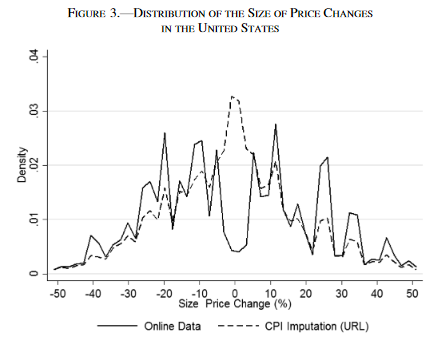
\includegraphics[width=.7\textwidth]{cavallo.png}
\caption{Cavallo's Price Distribution}
\label{fig:Cavallo_dist}
\end{figure}

\newpage
\begin{figure}
\centering
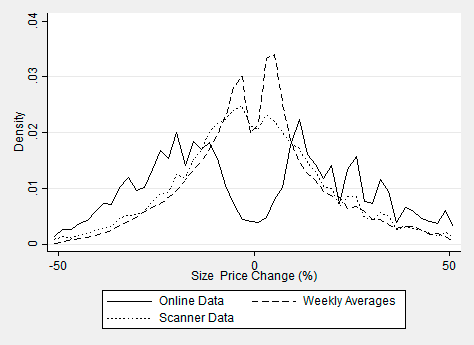
\includegraphics[width=.7\textwidth]{CavalloFig1.png}
\caption{Cavallo Figure 1}
\label{fig:CavalloFig_1}
\end{figure}

\newpage
\begin{figure}
\centering
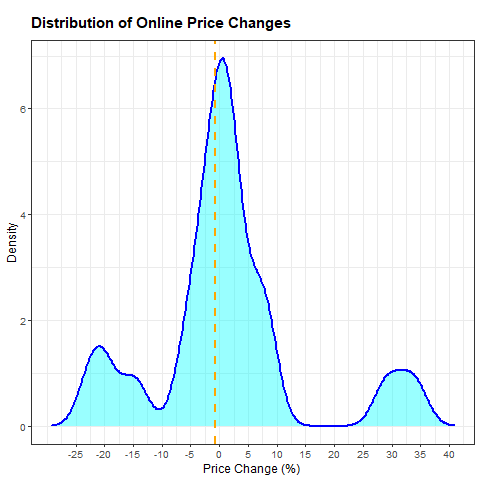
\includegraphics[width=.7\textwidth]{price_dist.png}
\caption{Price Distribution: Google SERP API}
\label{fig:price_dist}
\end{figure}

\newpage
\begin{figure}
\centering
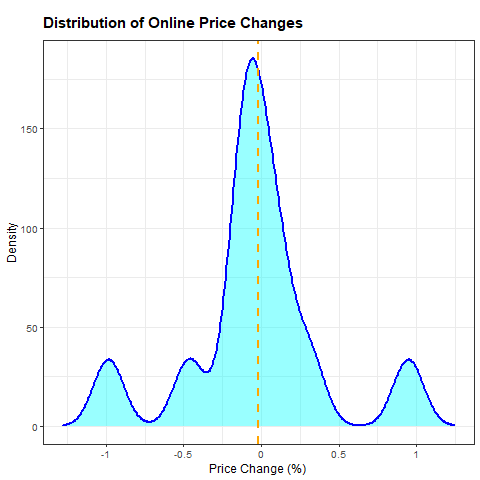
\includegraphics[width=.7\textwidth]{sub_dist.png}
\caption{Price Distribution: 14 day Sub Sample (Cavallo Data)}
\label{fig:sub_dist}
\end{figure}


%Python Graphs

\newpage
\begin{figure}
\centering
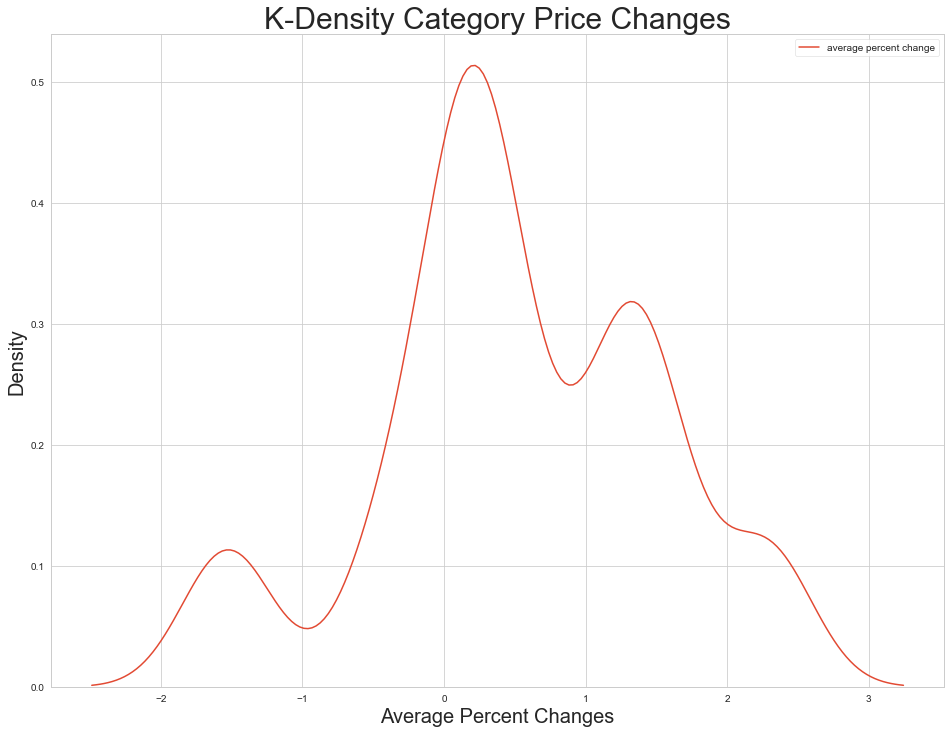
\includegraphics[width=.7\textwidth]{KDensity_Category_Price_Changes.png}
\caption{K-Density Plot of Walmart Data Price Changes by Category-Average}
\label{fig:avg_walmart_category}
\end{figure}

\newpage
\begin{figure}
\centering
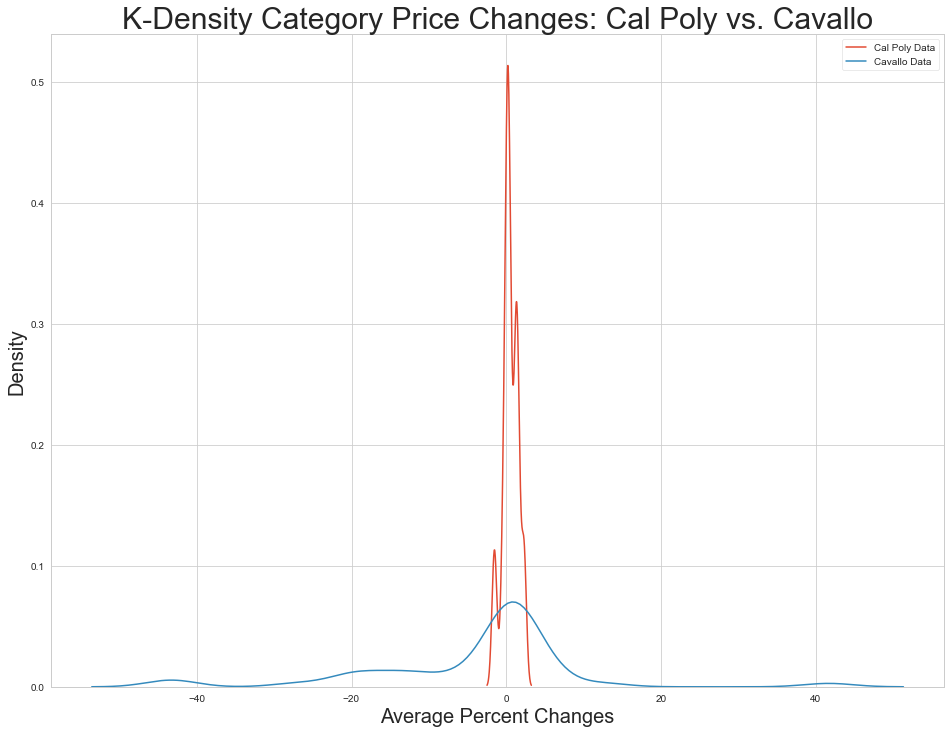
\includegraphics[width=.7\textwidth]{KDensity_Category_Price_Changes - Poly_vs_Cavallo - 2Week.png}
\caption{K-Density Plot Comparison of Walmart and Cavallo Data over Two-Week Period}
\label{fig:walmart-cavallo}
\end{figure}

\newpage
\begin{figure}
\centering
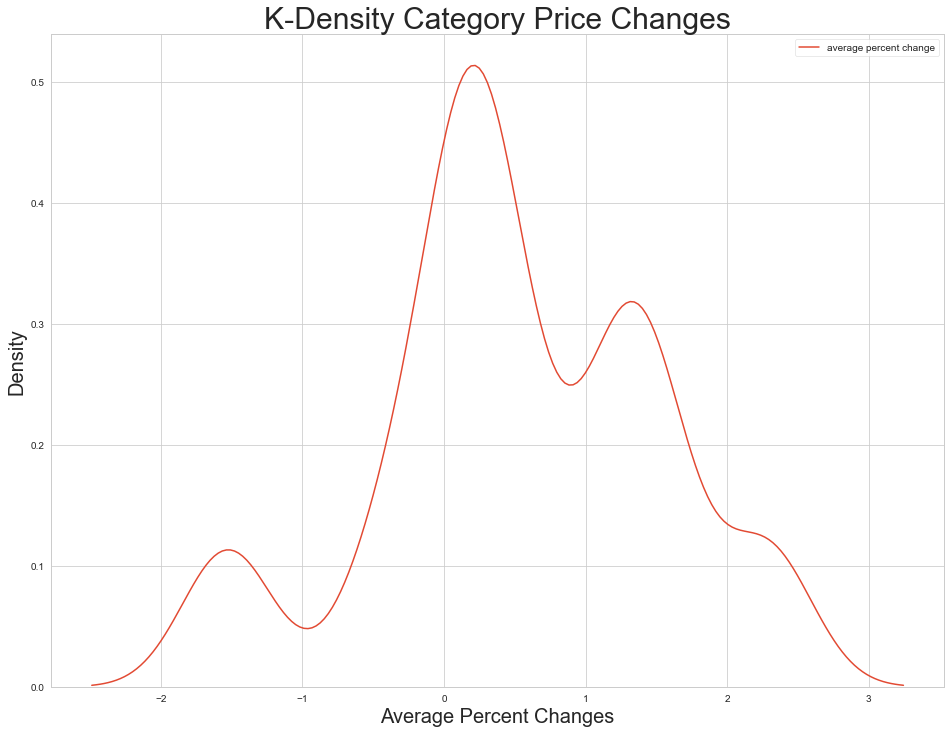
\includegraphics[width=.7\textwidth]{KDensity_Category_Price_Changes.png}
\caption{K-Density Plot of Walmart Data Price Changes by Individual Category}
\label{fig:indiv_walmart_category}
\end{figure}

\newpage
\begin{figure}
\centering
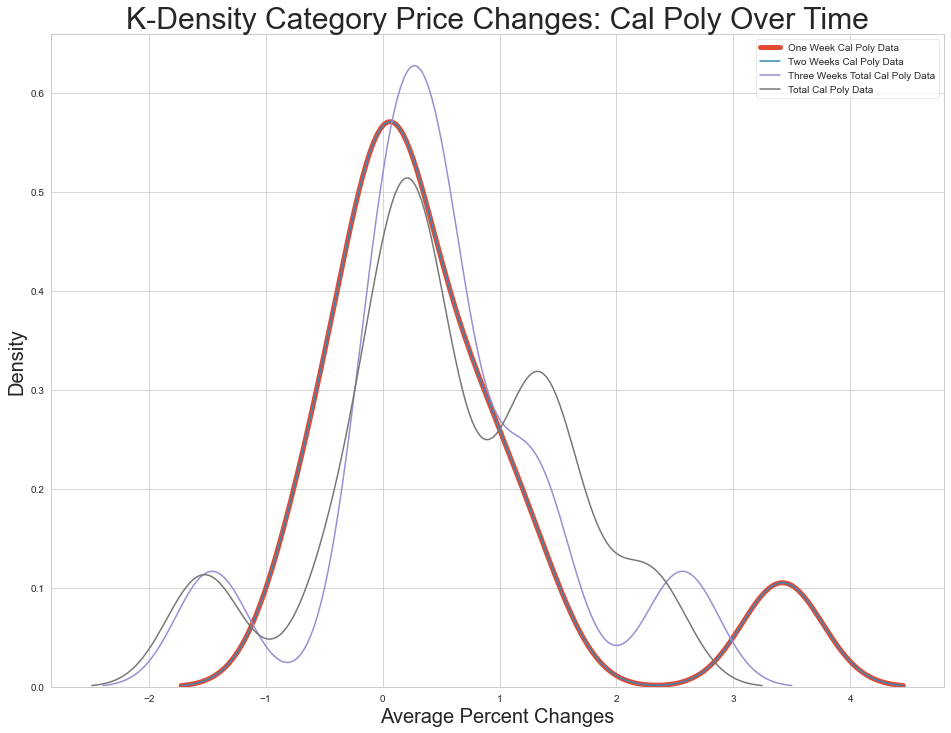
\includegraphics[width=.7\textwidth]{Walmart_Data_by_Length_of_Time.png}
\caption{K-Density Plot of Walmart Data by Duration}
\label{fig:walmart-duration}
\end{figure}



\begin{table}
\centering
\scalebox{1}{
  \begin{threeparttable}
    \caption{Database Description (Table 2 of \citet{Cavallo2015})}
     \begin{tabular}{lllllll}
        \toprule
         & {Google Shopping} & {Walmart (abbreviated)} & {Walmart (expanded)} \\
        \midrule
            Queries\tnote{a}       	& 5 	& 18 	& 78 \\
            Locations\tnote{b}	   	& 21 	& 1 	& 1 \\
            Avg. Daily Observations	& 2100  & 678	& 2303  \\        \bottomrule
     \end{tabular}
     
    \begin{tablenotes}
      \small
            \item[a] queries are strings used as search parameters for items (ie. the string typed into a search-bar)
            \item[b] locations are strings used to reference a geographical server from which the string takes place 
    \end{tablenotes}
  \end{threeparttable}
  }
\end{table}
\label{table:scrape1}

\begin{table}
\centering
\scalebox{1}{
  \begin{threeparttable}
    \caption{Database Description (Table 2 of \citet{Cavallo2015}) with New Walmart Data Column}
     \begin{tabular}{lllllll}
        \toprule
         & \( US \) & \( Argentina \) & \( Brazil \) & \( Chile \) & \( Columbia \) & \(Walmart \) \\
        \midrule
Retailers\tnote{a}                       & 4                                 & 1                             & 1                          & 1                         & 1                          & 1  \\
Observations (millions)\tnote{b}         & 28                                & 11                            & 10                         & 10                        & 4                          & 0.03  \\
Products (thousands)\tnote{c}            & 172                               & 28                            & 22                         & 24                        & 9                          & 4  \\
Days\tnote{d}                            & 865                               & 1,041                         & 1,026                      & 1,024                     & 992                        & 18  \\
Initial Date\tnote{e}                    & 03/08                             & 10/07                         & 10/07                      & 10/07                     & 11/07                      & 04/28/21  \\
Final Date\tnote{f}                      & 08/10                             & 08/10                         & 08/10                      & 08/10                     & 08/10                      & current  \\
Categories\tnote{g}                      & 49                                & 74                            & 72                         & 72                        & 59                         & 11  \\
URLs\tnote{h}                            & 16,188                            & 993                           & 322                        & 292                       & 123                        & 6,887  \\
Total missing observations (\%)\tnote{i} & 37                              & 32                            & 26                         & 33                        & 22                         & 0.04  \\ \hline
        \bottomrule
     \end{tabular}
     
    \begin{tablenotes}
      \small
      \item[a] number of retailers from which data is gathered 
      \item[b] total number of observations of price and metadata 
      \item[c] total number of unique products 
      \item[d] total number of days for which data was collected 
      \item[e] initial date of data collection 
      \item[f] final date of data collection 
      \item[g] total number of product categories 
      \item[h] total number of unique product page urls 
      \item[i] total percentage of products for which price data is missing 
    \end{tablenotes}
  \end{threeparttable}
  }
\end{table}
\label{table:cavallo1}





\end{document}